\question{考虑平面电磁波在两种线性各向同性介质的界面的反射和折射,设界面是无穷大光滑平面。根据麦克斯韦方程组和边值关系,分别对入射电场垂直入射面和平行入射面两种情形推导反射电场与入射电场的比、折射电场与入射电场的比,并给出反射率的表达式。请自行定义相关物理量的记号。}

    \begin{figure}[htbp]
        \centering
        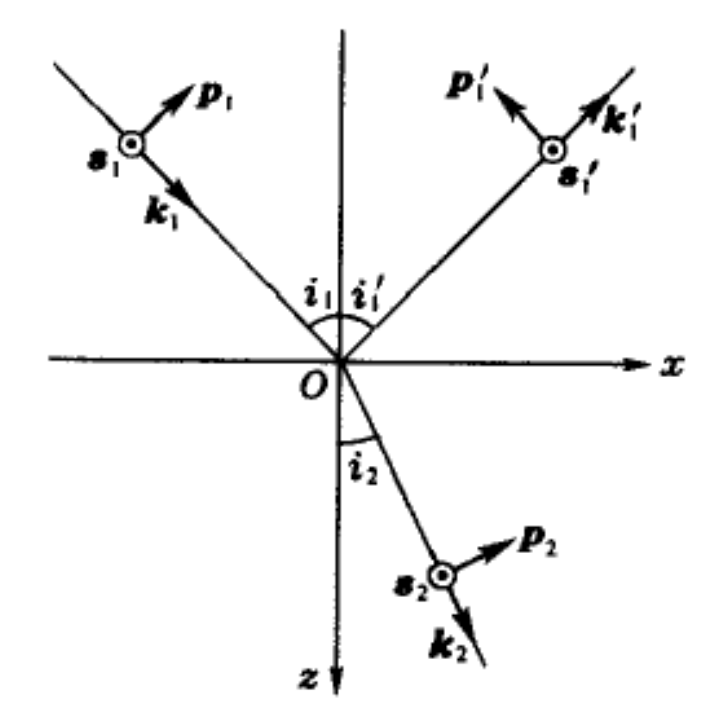
\includegraphics[width=6cm]{img/4.2/正交系.png}
        \caption{正方向定义}
        \label{4.2_fig:正方向定义}
    \end{figure}

    设入射波的单模平面波解为
    \equa{\e_i=\e_{i0}\exp{\i\kuohao{\k_i\cdot\x-\o_it}}\label{4.2_pm1}}
    设反射波的单模平面波解为
    \equa{\e_r=\e_{r0}\exp{\i\kuohao{\k_r\cdot\x-\o_rt}}\label{4.2_pm2}}
    设折射波的单模平面波解为
    \equa{\e_t=\e_{t0}\exp{\i\kuohao{\k_t\cdot\x-\o_tt}}\label{4.2_pm3}}
    设界面为\nota{z=0}平面,\nota{z<0}为介质1,\nota{z>0}为介质2,电磁波从介质1射向介质2。设入射角为\nota{\theta_i},反射角为\nota{\theta_r},折射角为\nota{\theta_t}。对于电场p波(电场偏振方向平行于入射面)、电场s波(电场偏振方向垂直于入射面)、波矢\nota{\k}的正方向定义如图\ref{4.2_fig:正方向定义}所示。
    
    电场的边值关系
    \equa{\bm{e}_z\times\kuohao{\e_i+\e_r}=\bm{e}_z\times\e_t\label{4.2_bianze}}
    要对任意\nota{\x\in\{z=0\}}成立,则(根据线性无关性)必须有
    \equa{\o_i=\o_r=\o_t=\o\label{4.2_边值关系1}}
    \equa{\bm{e}_z\times\k_i=\bm{e}_z\times\k_r=\bm{e}_z\times\k_t\label{4.2_边值关系2}}
    即
    \equa{k_i\sin\theta_i=k_r\sin\theta_r=k_t\sin\theta_t\label{4.2_k1}}
    在介质中有
    \equa{k_i=k_r=\o\sqrt{\mu_1\eps_1}\label{4.2_k2}}
    \equa{k_t=\o\sqrt{\mu_2\eps_2}\label{4.2_k3}}
    由(\ref{4.2_k1})(\ref{4.2_k2})(\ref{4.2_k3})得
    \equa{\theta_i=\theta_r\label{4.2_反射定律}}
    \equa{\sqrt{\mu_1\eps_1}\sin\theta_i=\sqrt{\mu_2\eps_2}\sin\theta_t\label{4.2_折射定律}}
    此即反射定律和折射定律。
    
    再考虑磁场的边值关系
    \equa{\bm{e}_z\times\kuohao{\h_i+\h_r}=\bm{e}_z\times\h_t\label{4.2_bianzh}}
    以及电磁波中磁场和电场的关系
    \equa{\h=\sqrt{\frac{\eps}{\mu}}\bm{e}_k\times\e\label{4.2_he}}
    
    如果电场偏振方向垂直于入射面(即s波)   将单模平面波解(\ref{4.2_pm1})(\ref{4.2_pm2})(\ref{4.2_pm3})以及反射定律(\ref{4.2_反射定律})代入(\ref{4.2_bianze})(\ref{4.2_bianzh})(\ref{4.2_he})中(尤其注意正方向如图\ref{4.2_fig:正方向定义}不要弄错)得
    \equa{
        \begin{pmatrix}
            1 &
            -1 \\
            \sqrt{\eps_1/\mu_1}\cos\theta_i &
            \sqrt{\eps_2/\mu_2}\cos\theta_t
        \end{pmatrix}
        \begin{pmatrix}
            E_r \\ E_t
        \end{pmatrix}
        =
        \begin{pmatrix}
            -1 \\ \sqrt{\eps_1/\mu_1}\cos\theta_i
        \end{pmatrix}
        E_i
    }
    解得
    \equa{
        \frac{E_r}{E_i}=
        \frac{\epmua\cos\theta_i-\epmub\cos\theta_t}{\epmua\cos\theta_i+\epmub\cos\theta_t}\label{4.2_s反射}
    }
    \equa{
        \frac{E_t}{E_i}=
        \frac{2\epmua\cos\theta_i}{\epmua\cos\theta_i+\epmub\cos\theta_t}
    }
    
    振幅反射率即(\ref{4.2_s反射}),强度反射率/能流密度反射率则为
    \equa{R=\kuohao{\frac{E_r}{E_i}}^2=\kuohao{\frac{\epmua\cos\theta_i-\epmub\cos\theta_t}{\epmua\cos\theta_i+\epmub\cos\theta_t}}^2}
    不过,需要注意对于折射而言,强度折射率和能流密度折射率是不同的,这里就不展开了。
    
    如果电场偏振方向平行于入射面(即p波)   将单模平面波解(\ref{4.2_pm1})(\ref{4.2_pm2})(\ref{4.2_pm3})以及反射定律(\ref{4.2_反射定律})代入(\ref{4.2_bianze})(\ref{4.2_bianzh})(\ref{4.2_he})中(尤其注意正方向如图\ref{4.2_fig:正方向定义}不要弄错)得
    \equa{
        \begin{pmatrix}
            \cos\theta_i &
            \cos\theta_t \\
            \epmua &
            -\epmub
        \end{pmatrix}
        \begin{pmatrix}
            E_r \\ E_t
        \end{pmatrix}
        =
        \begin{pmatrix}
            \cos\theta_i \\ -\epmua
        \end{pmatrix}
        E_i
    }
    解得
    \equa{
        \frac{E_r}{E_i}=
        \frac{-\epmua\cos\theta_t+\epmub\cos\theta_i}{\epmua\cos\theta_t+\epmub\cos\theta_i}\label{4.2_p反射}
    }
    \equa{
        \frac{E_t}{E_i}=
        \frac{2\epmua\cos\theta_i}{\epmua\cos\theta_t+\epmub\cos\theta_i}
    }
    
    振幅反射率即(\ref{4.2_p反射}),强度反射率/能流密度反射率则为
    \equa{R=\kuohao{\frac{E_r}{E_i}}^2=\kuohao{\frac{-\epmua\cos\theta_t+\epmub\cos\theta_i}{\epmua\cos\theta_t+\epmub\cos\theta_i}}^2}

\question{考虑电场平行入射平面的平面电磁波从真空入射到无穷大光滑玻璃平面,设玻璃折射率为\nota{n=1.5}。\label{4.2_题2}}

    \subquestion{根据菲涅耳公式,画出反射电场与入射电场的比作为入射角函数的函数曲线;画出折射电场与入射电场的比作为入射角函数的函数曲线。}
    
    \begin{tcolorbox}[breakable, size=fbox, boxrule=1pt, pad at break*=1mm,colback=cellbackground, colframe=cellborder]
    \prompt{In}{incolor}{in}{\boxspacing}
        \begin{matcode}   
            % para
            n1 = 1;
            n2 = 1.5;
            
            % prec
            i  = linspace(0, pi/2, 100);
            si = sin(i);
            ci = cos(i);
            st = n1 / n2 * si;
            ct = sqrt( 1 - (n1/n2)^2 * si.^2 );
            
            % calc
            R  = ( -n1 * ct + n2 * ci ) ./ ( n1 * ct + n2 * ci );
            T  = ( 2 * n1 * ci ) ./ ( n1 * ct + n2 * ci );
            
            % plot
            figure;
            plot(i, R, "LineWidth", 3, "Color", 'r');
            hold on;
            plot(i, T, "LineWidth", 3, "Color", 'b');
            legend('反射', '折射')
            xlabel('入射角 (rad)');
            ylabel('振幅比');
            xticks([0, pi/8, pi/4, pi/8*3 , pi/2]);
            xticklabels({'0', '\pi/8', '\pi/4', '3\pi/4', '\pi/2'});
            ylim([-1, 1]);
            set(gca, 'FontSize', 16);
            set(gca, 'LineWidth', 1);
            grid on;
        \end{matcode}
    \end{tcolorbox}
    
    \begin{figure}[htbp]
    \prompt{Out}{outcolor}{out}{\boxspacing}
        \centering
        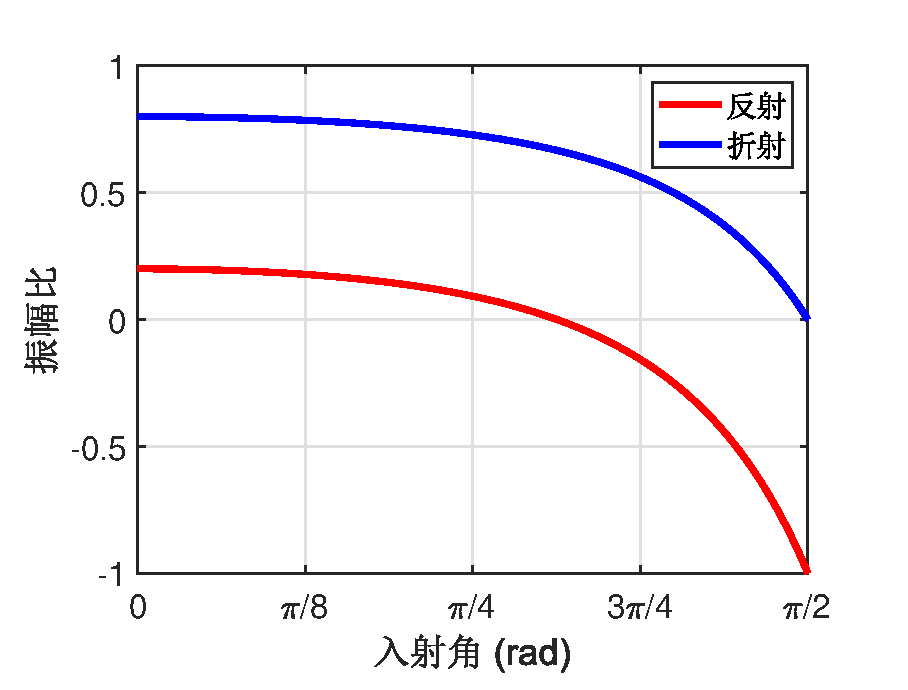
\includegraphics[width=10cm]{img/4.2/zwei.eps}
        \caption{振幅比随入射角的变化(从空气射入玻璃)}
        \label{4.2_fig:振幅比随入射角的变化(从空气射入玻璃)}
    \end{figure}
    
    \subquestion{求出布儒斯特角的数值。}
    
    可以用数值方法,从图\ref{4.2_fig:振幅比随入射角的变化(从空气射入玻璃)}中直接读出p波振幅反射比为0的入射角即布儒斯特角
    \equa{\theta_B=0.9828~\mathrm{rad}}
    
    也可以用解析的办法,令(\ref{4.2_p反射})取零,并考虑\nota{\mu_1\approx\mu_2}得
    \equa{\theta_i+\theta_t=\frac{\pi}{2}\label{4.2_tmp1}}
    又将折射定律(\ref{4.2_折射定律})改写为
    \equa{\sin\theta_i=n\sin\theta_t\label{4.2_tmp2}}
    由(\ref{4.2_tmp1})(\ref{4.2_tmp2})得
    \equa{\theta_B=\arctan n=0.9828~\mathrm{rad}}
    
\question{接上题,考虑平面光波从玻璃介质入射到玻璃和真空的无穷大光滑平面界面。求全反射角的数值。}

    可以用与题\ref{4.2_题2}类似的数值办法,找到强度反射比为1的入射角(这里以p波为例)
    
    \begin{tcolorbox}[breakable, size=fbox, boxrule=1pt, pad at break*=1mm,colback=cellbackground, colframe=cellborder]
    \prompt{In}{incolor}{in}{\boxspacing}
        \begin{matcode}   
            % para
            n1 = 1.5;
            n2 = 1;
            
            % prec
            i  = linspace(0, pi/2, 100);
            si = sin(i);
            ci = cos(i);
            st = n1 / n2 * si;
            ct = sqrt( 1 - (n1/n2)^2 * si.^2 );
            
            % calc
            R  = ( -n1 * ct + n2 * ci ) ./ ( n1 * ct + n2 * ci );
            T  = ( 2 * n1 * ci ) ./ ( n1 * ct + n2 * ci );
            R  = abs(R).^2;
            T  = abs(T).^2;
            
            % plot
            figure;
            plot(i, R, "LineWidth", 3, "Color", 'r');
            xlabel('入射角 (rad)');
            ylabel('p波强度反射率');
            xticks([0, pi/8, pi/4, pi/8*3 , pi/2]);
            xticklabels({'0', '\pi/8', '\pi/4', '3\pi/4', '\pi/2'});
            ylim([0, 1]);
            set(gca, 'FontSize', 16);
            set(gca, 'LineWidth', 1);
        \end{matcode}
    \end{tcolorbox}
    
    \begin{figure}[htbp]
    \prompt{Out}{outcolor}{out}{\boxspacing}
        \centering
        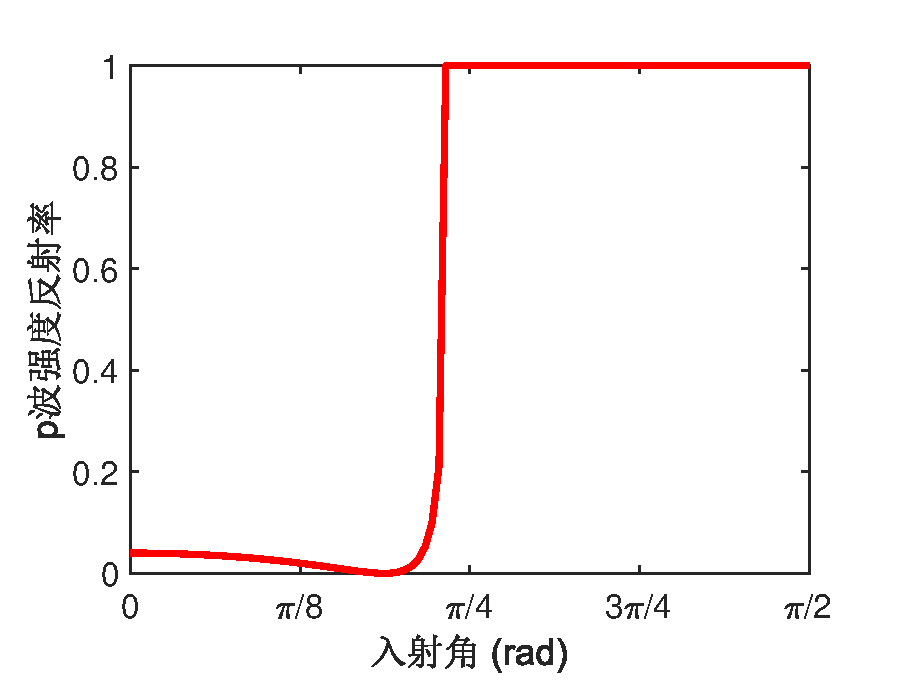
\includegraphics[width=10cm]{img/4.2/drei.eps}
        \caption{p波强度反射比随入射角的变化(从玻璃射入空气)}
        \label{4.2_fig:强度比随入射角的变化(从玻璃射入空气)}
    \end{figure}
    
    不过,需要注意的是这里考虑的应当是强度而非振幅,因为全反射会发生相移,使振幅反射/折射比为复数,直接画个实部是有失偏颇的。
    
    由此读出,全反射角
    \equa{\theta_c=0.7297~\mathrm{rad}}
    
    或者利用解析的办法也可容易地得出
    \equa{\theta_c=\arcsin\frac{1}{n}=0.7297~\mathrm{rad}}
    
\question{平面电磁波垂直射到金属表面上,试证明透入金属内部的电磁波能量全部变成焦耳热。}

    设金属界面为\nota{z=0}平面,\nota{z>0}为金属。设导体中波矢为
    \equa{\k=\bt+\i\ap=(\beta+\i\alpha)\bm{e}_z=k\bm{e}_z}
    金属中电场平面波
    \equa{\e=\e_0\exp{\i\kuohao{kz-\o t}}\label{4.2_4.1}}
    磁场波可由电场计算
    \equa{\h=\frac{1}{\o\mu}\k\times\e\label{4.2_4.2}}
    
    由(\ref{4.2_4.1})(\ref{4.2_4.2})计算进入金属界面的平均能流密度
    \equa{\langle\bm{S}\rangle = \frac{1}{2}\mathrm{Re}\kuohao{\e^*\times\h}=\frac{\beta}{2\o\mu}E_0^2\bm{e}_z\label{4.2_res1}}
    
    而根据欧姆定律
    \equa{\j=\sigma\e}
    则单位面积对应的焦耳热功率为
    \equa{\langle P\rangle=\int_0^\infty\frac{1}{2}\mathrm{Re}\kuohao{\j^*\times\e}\d z=\frac{\sigma E_0^2}{4\alpha}\label{4.2_res2}}
    由于垂直入射,有
    \equa{\alpha\beta=\frac{1}{2}\o\mu\sigma\label{4.2_res3}}
    由(\ref{4.2_res1})(\ref{4.2_res2})(\ref{4.2_res3})知
    \equa{\langle S\rangle=\langle P\rangle}
    
\question{平面电磁波由真空倾斜入射到导电介质表面上,入射角为\nota{\theta_1}。求导电介质中电磁波的相速度和衰减长度。若导电介质为金属,结果如何?}
    
    设平面单模波解如(\ref{4.2_pm1})(\ref{4.2_pm2})(\ref{4.2_pm3}),得其边值关系
    (\ref{4.2_边值关系1})(\ref{4.2_边值关系2})。这里只需要把折射波波矢\nota{\k_t}改写为复矢量
    \equa{\k_t=\bt+\i\ap\label{4.2_fu}}
    取xz平面为入射平面,记\nota{\theta_1=\theta_i}。由(\ref{4.2_边值关系2})(\ref{4.2_fu})得
    \equa{\alpha_x=\alpha_y=\beta_y=0\label{4.2_5.3}}
    \equa{\beta_x=k_i\sin\theta_i=\frac{\o}{c}\sin\theta_1\label{4.2_5.4}}
    
    导电介质中有亥姆霍兹方程
    \equa{\nabla^2\e_t+\o^2\mu\kuohao{\eps+\i\frac{\sigma}{\o}}\e_t=0\label{4.2_haim}}
    将(\ref{4.2_pm3})(\ref{4.2_fu})代入(\ref{4.2_haim})得
    \equa{\beta^2-\alpha^2=\o^2\mu\eps\label{4.2_5.1}}
    \equa{\ap\bt=\frac{1}{2}\o\mu\sigma\label{4.2_5.2}}
    
    由(\ref{4.2_5.3})(\ref{4.2_5.4})(\ref{4.2_5.1})(\ref{4.2_5.2})得
    \equa{\kuohao{\frac{\o}{c}\sin\theta_1}^2+\beta_z^2-\alpha_z^2=\o^2\mu\eps}
    \equa{\alpha_z\beta_z=\frac{1}{2}\o\mu\sigma}
    解得
    \equa{\beta_z^2=\frac{1}{2}\kuohao{\mu\eps\o^2-\frac{\o^2}{c^2}\sin^2\theta_1}+\frac{1}{2}\fkuohao{\kuohao{\mu\eps\o^2-\frac{\o^2}{c^2}\sin^2\theta_1}^2+\kuohao{\mu\sigma\o}^2}^\frac{1}{2}}
    \equa{\alpha_z^2=-\frac{1}{2}\kuohao{\mu\eps\o^2-\frac{\o^2}{c^2}\sin^2\theta_1}+\frac{1}{2}\fkuohao{\kuohao{\mu\eps\o^2-\frac{\o^2}{c^2}\sin^2\theta_1}^2+\kuohao{\mu\sigma\o}^2}^\frac{1}{2}}
    则相速度为
    \equa{v=\frac{\o}{\beta}=\frac{\o}{\sqrt{\beta_x^2+\beta_z^2}}}
    穿透深度为
    \equa{\delta=\frac{1}{\alpha}=\frac{1}{\sqrt{\alpha_z^2}}}
    
    若导电介质为金属,则有良导体条件
    \equa{\frac{\sigma}{\o\eps}\gg 1}
    从而
    \equa{k_t^2=\i\o\mu\sigma\kuohao{1-\i\frac{\o\eps}{\sigma}}\approx\i\o\mu\sigma}
    于是
    \equa{\beta^2-\alpha^2\approx0}
    \equa{\alpha_z\beta_z=\frac{1}{2}\o\mu\sigma=\frac{1}{2}\o^2\mu_0\eps_0\frac{\sigma}{\o\eps_0}\gg\frac{1}{2}\kuohao{\frac{\o}{c}}^2}
    即
    \equa{\alpha_z\beta_z\gg\beta_x^2}
    故得近似解
    \equa{\alpha\approx\beta\approx\sqrt{\frac{\o\mu\sigma}{2}}}
    则相速度为
    \equa{v=\frac{\o}{\beta}=\sqrt{\frac{2\o}{\mu\sigma}}}
    穿透深度为
    \equa{\delta=\frac{1}{\alpha}=\sqrt{\frac{2}{\o\mu\sigma}}}
